\lab{PageRank Algorithm}{PageRank Algorithm}
\label{lab:PageRank}
\objective{Model a network as a graph and implement the PageRank algorithm based on this model. 
Use PageRank to predict the rankings of sports teams. }

\begin{comment}
When you enter keywords into Google's search engine, Google finds every page containing your keywords and lists the pages in order of their \emph{rank}.
The rank of a page reflects many factors, including how often the page is visited and how connected it is to other pages.
\end{comment}
As of 2013, the PageRank algorithm is one of over 200 algorithms that Google uses to determine the \emph{rank}, or relative importance, of a webpage.
Named for Larry Page, cofounder of Google, this algorithm ranks pages based on how many other pages link to them.

\begin{comment}
The PageRank algorithm is also used in applications other than internet search engines.
For example, it has been used to rank graduate institutions and the impact factor of journals, and it has been used in some biological applications.
\end{comment}

\section*{The Internet as a Graph}
The PageRank algorithm models the internet with a directed graph. 
Each webpage is a node, and there is an edge from node $i$ to node $j$ if page $i$ links to page $j$.
Let $\In(i)$ be the websites linking to page $i$ and let $\Out(i)$ be the websites that page $i$ links to. 
That is, $\In(i)$ is the set of nodes with an arrow to node $i$, and $\Out(i)$ is the set of nodes with an arrow from node $i$.
An example is illustrated in Figure \ref{fig:network1}.

\begin{figure}
\centering
\begin{tikzpicture}[node distance=1.75cm, thick ]

\node[draw=none](2)[]{2};
\node[draw=none](3)[right of=2]{3};
\node[draw=none](4)[right of=3]{4};
\node[draw=none](5)[right of=4]{5};
\node[draw=none](6)[right of=5]{6};
\node[draw=none](1)[above of=3]{1};
\node[draw=none, node distance=2.5cm](0)[right of=1]{0};
\node[draw=none](dummy)[above right of=0]{};
\node[draw=none, node distance=.5cm](7)[below 
	of=dummy]{7};

\foreach \x/\y in {3/2, 4/5, 5/6, 1/0, 3/0, 4/0, 5/0} \draw[->, 
	>=stealth'](\x)--(\y);
\draw[->, >=stealth'](6)--(0);
\draw[->, >=stealth', shorten >= .1cm](7)edge[bend left=20](0);
\draw[->, >=stealth', shorten <= .1cm](0)edge[bend left=20](7);
\draw[->, >=stealth', shorten <= .1cm](3)edge[bend right=40](6.9,-.25);
\draw[->, >=stealth', shorten <= .1cm](4)edge[bend right](6);



\end{tikzpicture}

\caption{This directed graph describes the links between 8 webpages. In this example, $\In(0)=\{1,3,4,5,6,7\}$ and $\Out(0)=\{7\}$.}
\label{fig:network1}
\end{figure}

The PageRank algorithm ranks pages by how many others link to them.
A link from a more important page counts more than one from a less important page.
For example, in Figure \ref{fig:network1} we would expect node 0 to have a very high rank because every other node links to it. 
Consequently, we would expect node 7 to have a fairly high rank because node 0 links to it, even though node 0 is the only node to do so.

\section*{The PageRank Algorithm}
The PageRank algorithm assumes that a surfer chooses a starting webpage randomly.
Then, if the surfer is at page $i$, they randomly select a page from $\Out(i)$ to visit next.
This means that the surfer's chance of being on page $i$ at time $t$ is determined by where they were at time $t-1$.

Suppose the internet has $N$ webpages, and let $p_i(t)$ be the likelihood that the surfer is on page $i$ at time $t$.
Then the probabilities $p_i(t)$ are given by
\begin{equation}\label{equ:pr1}
p_i(0)=\frac{1}{N} \qquad p_i(t+1) = \sum_{j \in \In(i)} \frac{p_j(t)}{\abs{\Out(j)}}.
\end{equation}

For example, in Figure \ref{fig:network1} we have $N=8$, and 
\[
p_6(t+1)=\frac{p_3(t)}{3}+\frac{p_4(t)}{3} + \frac{p_5(t)}{2}.
\]

\subsection*{Refining the Model: Pages with No Outbound Links}
A node with no outbound links, such as node 2 in Figure \ref{fig:network1}, is called a \emph{sink}. 
According to our model, if the surfer ever visits a sink, they will stay there forever.

This is not very realistic; in this situation, a person would likely select another webpage at random and begin surfing again.
Hence, in our model we replace sinks with nodes linking to every other page. 
This means we modify Figure \ref{fig:network1} (where node 2 is a sink) to look like Figure \ref{fig:network2}.

\begin{figure}
\centering
\begin{tikzpicture}[node distance=1.75cm, >=stealth', thick]

\node[draw=none](2)[]{2};
\node[draw=none](3)[right of=2]{3};
\node[draw=none](4)[right of=3]{4};
\node[draw=none](5)[right of=4]{5};
\node[draw=none](6)[right of=5]{6};
\node[draw=none](1)[above of=3]{1};
\node[draw=none, node distance=2.5cm](0)[right of=1]{0};
\node[draw=none](dummy)[above right of=0]{};
\node[draw=none, node distance=.5cm](7)[below 
	of=dummy]{7};


\draw[->, color=black!35!](2)--(1);
\draw[->, color=black!35!, shorten >= .2cm](2)--(0);
\foreach \x/\y in {2/3, 2/4, 2/5} \draw[->, color=black!35!](\x)
	edge[bend right](\y);

\draw[->, shorten <= .1cm, color=black!35!](2)edge[bend right=50](7,-.35);
\draw[->, shorten <= .1cm](3)edge[bend right=40](6.9,-.25);
\draw[->, shorten <= .1cm](4)edge[bend right](6);
\draw[->, shorten <=.1cm, color=black!35!](2)edge[bend left=40](7);

\draw[->, shorten >= .1cm](7)edge[bend left=20](0);
\draw[->, shorten <= .1cm](0)edge[bend left=20](7);

\foreach \x/\y in {3/2, 4/5, 5/6, 1/0, 3/0, 4/0, 5/0} \draw[->, 
	>=stealth'](\x)--(\y);
\draw[-> ](6)--(0);

\end{tikzpicture}

\caption{Here Figure \ref{fig:network1} has been modified to guarantee that page 2 is no longer a sink. A new link has been added from page 2 to every other page (the added links are grey).}
\label{fig:network2}
\end{figure}

\subsection*{Refining the Model: Adding Boredom}
The equations in \eqref{equ:pr1} assume that the current page must link to the next page.
However, the model is more realistic if we assume that the surfer sometimes gets bored and randomly picks a new starting page.
We will denote the probability that a surfer stays interested at step $t$ by a constant $d$, called the \emph{damping factor}.
Then the probability that the surfer gets bored at time $t$ is $1-d$.
The formulas in \eqref{equ:pr1} then become
\begin{equation}\label{equ:pr2}
p_i(0)=\frac{1}{N} \qquad p_i(t+1) = d\sum_{j \in \In(i)} \frac{p_j(t)}{\abs{\Out(j)}}+\frac{1-d}{N} .
\end{equation}

\subsection*{Matrix Form of the PageRank Algorithm}
We can rewrite \eqref{equ:pr2} as the matrix equation
\begin{equation}\label{equ:pr3}
\mathbf{p}(0)=\frac{1}{N}\mathbf{1} \qquad \mathbf{p}(t+1) = dK\mathbf{p}(t) + \frac{1-d}{N}\mathbf{1}
\end{equation}
where $\mathbf{p}(t)=(p_1(t), p_2(t), \ldots, p_N(t))^T$, 
$\mathbf{1}$ is a vector of $N$ ones, 
and $K$ is defined by
\[K_{ij} = \begin{cases} \frac{1}{\abs{\Out(j)}} & \mbox{ if j links to i} \\
	0 & \mbox{ otherwise.} \end{cases}\]


\subsection*{Defining Page Rank}
As given by the PageRank algorithm, the \emph{rank} of page $i$ is
\[p_i = \lim_{t\to \infty} p_i(t).\]
In other words, the page ranks are the steady state of the modified Markov chain defined in \eqref{equ:pr3}.



\section*{Implementation in Python}


The adjacency matrix $A$ of a directed graph has $A_{ij}=1$ if there is an edge from node $i$ to node $j$, and $A_{ij}=0$ otherwise.
The adjacency matrix of the graph in Figure \ref{fig:network1} is defined below.
We use a code environment to describe $A$ so you can easily use this example to debug the problems in this lab.
\begin{lstlisting}
A = np.array([[ 0,  0,  0,  0,  0,  0,  0,  1],
              [ 1,  0,  0,  0,  0,  0,  0,  0],
              [ 0,  0,  0,  0,  0,  0,  0,  0],
              [ 1,  0,  1,  0,  0,  0,  1,  0],
              [ 1,  0,  0,  0,  0,  1,  1,  0],
              [ 1,  0,  0,  0,  0,  0,  1,  0],
              [ 1,  0,  0,  0,  0,  0,  0,  0],
              [ 1,  0,  0,  0,  0,  0,  0,  0]])
\end{lstlisting}

\begin{problem}
Write the following function that creates a sparse adjacency matrix from a file.
\begin{lstlisting}
def to_matrix( filename, n ):
    ''' Return the nxn adjacency matrix described by the file.
    
    INPUTS:
    filename - Name of a .txt file describing a directed graph. Lines 
    		    describing edges should have the form 
				'<from node>\t<to node>'. 
				The file may also include comments.
    n		- The number of nodes in the graph described by datafile
    
    RETURN:
    Return a SciPy sparse `dok_matrix'.
    '''
\end{lstlisting}
Hints:
\begin{enumerate}
\item The file \texttt{datafile.txt} included with this lab describes the matrix in Figure \ref{fig:network1} and has the adjacency matrix \li{A} given above. 
You may use it to test your function.

\item You can open a file in Python using the \li{with} syntax. 
Then, you can iterate through the lines using a \li{for} loop.
Here is an example.
\begin{lstlisting}
# Open `datafile.txt' for read-only
with open('./datafile.txt', 'r') as myfile:
    for line in myfile:
        print line
\end{lstlisting}

\item Here is an example of how to process a line of the form in \li{datafile}.
\begin{lstlisting}
>>> line = '0\t4\n'
# strip() removes trailing whitespace from a line.
# split() returns a list of the space-separated pieces of the line.
>>> line.strip().split()
['0', '4']
\end{lstlisting}

\item Rather than testing for lines of \texttt{datafile.txt} that contain comments, put all your string operations in a \li{try} block with an \li{except} block following.
\end{enumerate}
\end{problem}

\begin{info}
It makes sense to initialize $A$ as a sparse matrix, since $A$ is mostly zeros. To make the coding easier, throughout the rest of the lab the algorithms will be coded using non-sparse matrices. Don't forget, however, that in a real-world sparse adjacency matrices are generally much more time-efficient than dense matrices. 

To convert from a sparse to a non-sparse matrix, use the syntax \li{A.todense()}.
\end{info}

The next step is to compute $K$ from \eqref{equ:pr3}. 
A good strategy for computing $K$ comes from writing
\[
K = (D^{-1}A)^T
\]
where $A$ is the adjacency matrix of the directed graph representing the internet and $D$ is a diagonal matrix with $D_{jj}=\abs{\Out(j)}$.
Modify $A$ so that rows corresponding to sinks have all ones instead of all zeros.
For Figure \ref{fig:network2}, the modified adjacency matrix is defined below.
\begin{lstlisting}
Am = np.array([[ 0,  0,  0,  0,  0,  0,  0,  1],
               [ 1,  0,  0,  0,  0,  0,  0,  0],
               [ 1,  1,  1,  1,  1,  1,  1,  1],
               [ 1,  0,  1,  0,  0,  0,  1,  0],
               [ 1,  0,  0,  0,  0,  1,  1,  0],
               [ 1,  0,  0,  0,  0,  0,  1,  0],
               [ 1,  0,  0,  0,  0,  0,  0,  0],
               [ 1,  0,  0,  0,  0,  0,  0,  0]])
\end{lstlisting}


The matrix $D$ is easily obtained by summing the rows of $A$. 
Although  $K=(D^{-1}A)^T$, it is better practice to only store the diagonal entries of $D$ as a vector, and then use array broadcasting to divide $A$ by $D$.

Notice that we need to transpose $D^{-1}A$ to get $K$. This is because $D^{-1}A$ is \emph{row stochastic} (meaning that  the rows sum to 1), but we need to multiply \emph{column stochastic} matrices (where the columns sum to 1) To make $K$ be column stochastic, we have to take a transpose.

For Figure \ref{fig:network2}, the matrix $K$ is as follows.

\begin{lstlisting}
K = np.array([[ 0   ,  1   ,  1./8,  1./3,  1./3,  1./2,  1   ,  1   ],
              [ 0   ,  0   ,  1./8,  0   ,  0   ,  0   ,  0   ,  0   ],
              [ 0   ,  0   ,  1./8,  1./3,  0   ,  0   ,  0   ,  0   ],
              [ 0   ,  0   ,  1./8,  0   ,  0   ,  0   ,  0   ,  0   ],
              [ 0   ,  0   ,  1./8,  0   ,  0   ,  0   ,  0   ,  0   ],
              [ 0   ,  0   ,  1./8,  0   ,  1./3,  0   ,  0   ,  0   ],
              [ 0   ,  0   ,  1./8,  1./3,  1./3,  1./2,  0   ,  0   ],
              [ 1   ,  0   ,  1./8,  0   ,  0   ,  0   ,  0   ,  0   ]])
\end{lstlisting}
\begin{problem}
Write a function that computes the K matrix given an adjacency matrix.
\begin{enumerate}
\item Compute the diagonal matrix $D$.
\item Compute the modified adjacency matrix where the rows corresponding to sinks all have ones instead of zeros.
\item Compute $K$ using array broadcasting.
\end{enumerate}
\end{problem}


\subsection*{Solving for the Page Ranks}
There are several ways to solve for $\lim_{t \to \infty} \mathbf{p}(t)$.
\subsubsection*{Algebraic Method}
One possibility is to assume the modified Markov chain has a steady state $\mathbf{p}$ and solve for it algebraically:
\begin{equation}\label{equ:matrix_solve}
(I-dK)\mathbf{p} = \frac{1-d}{N} \mathbf{1}.
\end{equation}

We can use SciPy's solver to find the page ranks of the network in Figure \ref{fig:network2}.
\begin{lstlisting}
>>> from scipy import linalg as la
>>> I = np.eye(8)
>>> d = .85
>>> la.solve(I-d*K, ((1-d)/8)*np.ones(8))
array([ 0.43869288,  0.02171029,  0.02786154,  0.02171029,  0.02171029,
        0.02786154,  0.04585394,  0.39459924])
\end{lstlisting}
As expected, node 0 has the highest rank, approximately equal to .44. 
Node 7 has a higher rank than node 6, even though $\In(7)=1$ and $\In(6)=3$. 
This is because node 7's single in-edge comes from a node that has a very high rank (node 0).

\subsubsection*{Iterative Method}
Solving the system in \eqref{equ:matrix_solve} is feasible for our small working example, but this is not an efficient strategy for very large systems.

One option for large systems is an iterative method. 
Starting with a guess for $\mathbf{p}(0)$, we iterate on Equation \eqref{equ:pr3} until $\norm{\mathbf{p}(t)-\mathbf{p}(t-1)}$ is sufficiently small. 
At this point we assume we have reached the steady state.


\begin{problem}
\label{prob:pagerank_dense_iter}
Implement the function below, using the iterative method to find the steady state of the PageRank algorithm.
When the argument \li{N} is not \li{None}, work with only the upper $N \times N$ portion of the array \li{adj}.
Test your function against the example in the lab.
\begin{lstlisting}
def iter_solve( adj, N=None, d=.85, tol=1E-5):
    '''
    Return the page ranks of the network described by 'adj' using the iterative method.    
    
    INPUTS:
    adj - A NumPy array representing the adjacency matrix of a directed 
            graph
    N     - Restrict the computation to the first `N` nodes of the graph. 
            Defaults to N=None; in this case, the entire matrix is used.
    d     - The damping factor, a float between 0 and 1. 
            Defaults to .85.
    tol  - Stop iterating when the change in approximations to the 
            solution is less than `tol'. Defaults to 1E-5.    
            
    OUTPUTS:
    Return the approximation to the steady state of p.
    '''
\end{lstlisting}
Hints:
\begin{enumerate}
\item Try making your initial guess for $\mathbf{p}(0)$ a random vector.
\item NumPy can do unexpected things with the dimensions when performing matrix-vector multiplication.
When debugging, check at each iteration that all arrays have the dimensions you expect.
\end{enumerate}
\end{problem}

\subsubsection*{Eigenvalue Method}
Another way to solve this problem is to make it into an eigenvalue problem. 
Let $E$ be an $N \times N$ matrix of ones; then $E\mathbf{p}(t) = \mathbf{1}$. 
Hence, the matrix equation \eqref{equ:pr3} for $\mathbf{p}(t+1)$ becomes
\[\mathbf{p}(t+1) = \Big(dK + \frac{1-d}{N}E\Big)\mathbf{p}(t).\]
If we write $B = dK + \frac{1-d}{N}E$, this simplifies to $\mathbf{p}(t+1) = B\mathbf{p}(t).$
Thus, the steady state $\mathbf{p}(t)$ is an eigenvector of $B$ corresponding to the eigenvalue 1.

The columns of $B$ sum to 1, and the entries of $B$ are strictly positive (because the entries of $E$ are all positive).
With these hypotheses, the Perron-Frobenius theorem says that 1 is the unique eigenvalue of B of largest magnitude, and the corresponding eigenvector is unique.
In this case, the ``iterative method'' described above is just the power method for finding the eigenvector corresponding to a dominant eigenvalue, introduced in the lab on eigensolvers. %TODO: make sure the reference to another lab is accurate.

We can also compute $\mathbf{p}$ using eigenvalue solvers in SciPy.

%TODO: the output from scipy.linalg.eig is not very accurate, even for the small example in this lab.
\begin{problem}
Implement the function below, using the eigenvalue method to find the steady state of the PageRank algorithm.
\begin{lstlisting}
def eig_solve( adj, N=None, d=.85):
    '''
    Return the page ranks of the network described by `adj`.
    
    INPUTS:
    adj - A NumPy array representing the adjacency matrix of a directed 
            graph
    N     - Restrict the computation to the first `N` nodes of the graph. 
            Defaults to N=None; in this case, the entire matrix is used.
    d     - The damping factor, a float between 0 and 1. 
            Defaults to .85.
    
    OUTPUTS:
    Return the approximation to the steady state of p.
    '''
\end{lstlisting}
Hint: Review the techniques from the Markov chain section of Lab \ref{lab:EigSolve}.
\end{problem}

\section*{Ranking Teams}
This ranking algorithm can be applied not only to webpages, but to any problem with a directed graph structure. 
One such application is ranking sports teams.

Suppose we have data about a collection of sports teams, including which teams played each other and who won each match. 
We can model this as a directed graph. Each node in the graph represents a team.
An edge between two nodes points from the losing team to the winning team. 
If two teams never played each other, there is no edge between them.
Wins and losses do not cancel out; if BYU and Boise played twice, and each team won once, then there is an edge from BYU to Boise and another edge from Boise to BYU. TODO: add a picture.

To simplify our model, edges are not weighted. So if Duke ever beat Harvard, no matter whether they beat them once or 5 times, there is only one edge pointing from Harvard to Duke. 

The key here is that edges tend to lead from worse teams to better teams. 
So by starting with some team and randomly following edges, we should end up visiting better teams more often. 
This is reminiscent of the PageRank algorithm! Given an appropriate dataset, we can use PageRank to estimate team rankings.  

Note that in this scenario, the parameter $d$ no longer represents boredom. 
It allows us to jump randomly from one team to another, so it could represent a surprise upset, or the random outcome of a game between two teams who have never played each other.

\begin{problem}
By applying the PageRank algorithm to win-loss data from the 2013 NCAA basketball season, produce a comparative ranking of the teams.
\begin{enumerate}
\item The file  \texttt{ncaa2013.csv} contains data on over 5000 basketball games. 
The first line is a header.
After the header, each line represents a game and has the winning team followed by the losing team (there are no ties in basketball). 

Load this file and use it to create the adjacency matrix $A$, where $A_{ij} = 1$ if team $j$ beat team $i$. 
Make sure to ignore the header line.
You will need some way of mapping from team names to the integers and vice versa.
\item Use the iterative method from Problem \ref{prob:pagerank_dense_iter} with $d = 0.7$ to find the steady state. 
The steady-state solution is your vector of ranks. 
\item Return the ranks sorted from largest to smallest, and the corresponding list of teams sorted from ``best'' to ``worst''. 
\end{enumerate}
Hints:
\begin{enumerate}
\item The code below may be helpful for processing the .csv file:
\begin{lstlisting}
>>> with open('./ncaa2013.csv', 'r') as ncaafile:
>>>     ncaafile.readline() #reads and ignores the header line
>>>     for line in ncaafile:
>>>         teams = line.strip().split(',') #split on commas
>>>         print teams
>>> ['Middle Tenn St', 'Alabama St']
>>> ...
>>> ['Mississippi', 'Florida']
\end{lstlisting}
\item Before creating the adjacency matrix, you can get all the unique teams by running through all the matches once and adding every team to a set. 
Next, count the number of unique teams and initialize $A$ to be the right size.
Try using dictionaries, lists, or both to map numbers to teams and teams to numbers and fill in $A$. 
There is more than one right way to do this.
\item The function \li{np.argsort()} will be useful for sorting the ranks and teams.
\item There should be 347 teams. PageRank should predict that the top five ranked teams are Duke, Butler, Louisville, Illinois, and Indiana (in that order). Use this to check your results.
\end{enumerate}
\end{problem}

\section*{Optional: SNAP Datasets}
The SNAP graph library, located at \url{http://snap.stanford.edu/data/index.html}, provides a variety of medium sized data sets for public use.
These datasets have to do with networks, including road systems, social networks, and online communities. There are some interesting resources here for those wanting to experiment further with the PageRank algorithm on different datasets.
\begin{comment}
The \li{matplotlib.pyplot.spy} command on the adjacency matrix from a SNAP data set yielded the plot shown in Figure \ref{fig:WebSparse}
\end{comment}

\begin{comment}
\begin{figure}
\centering
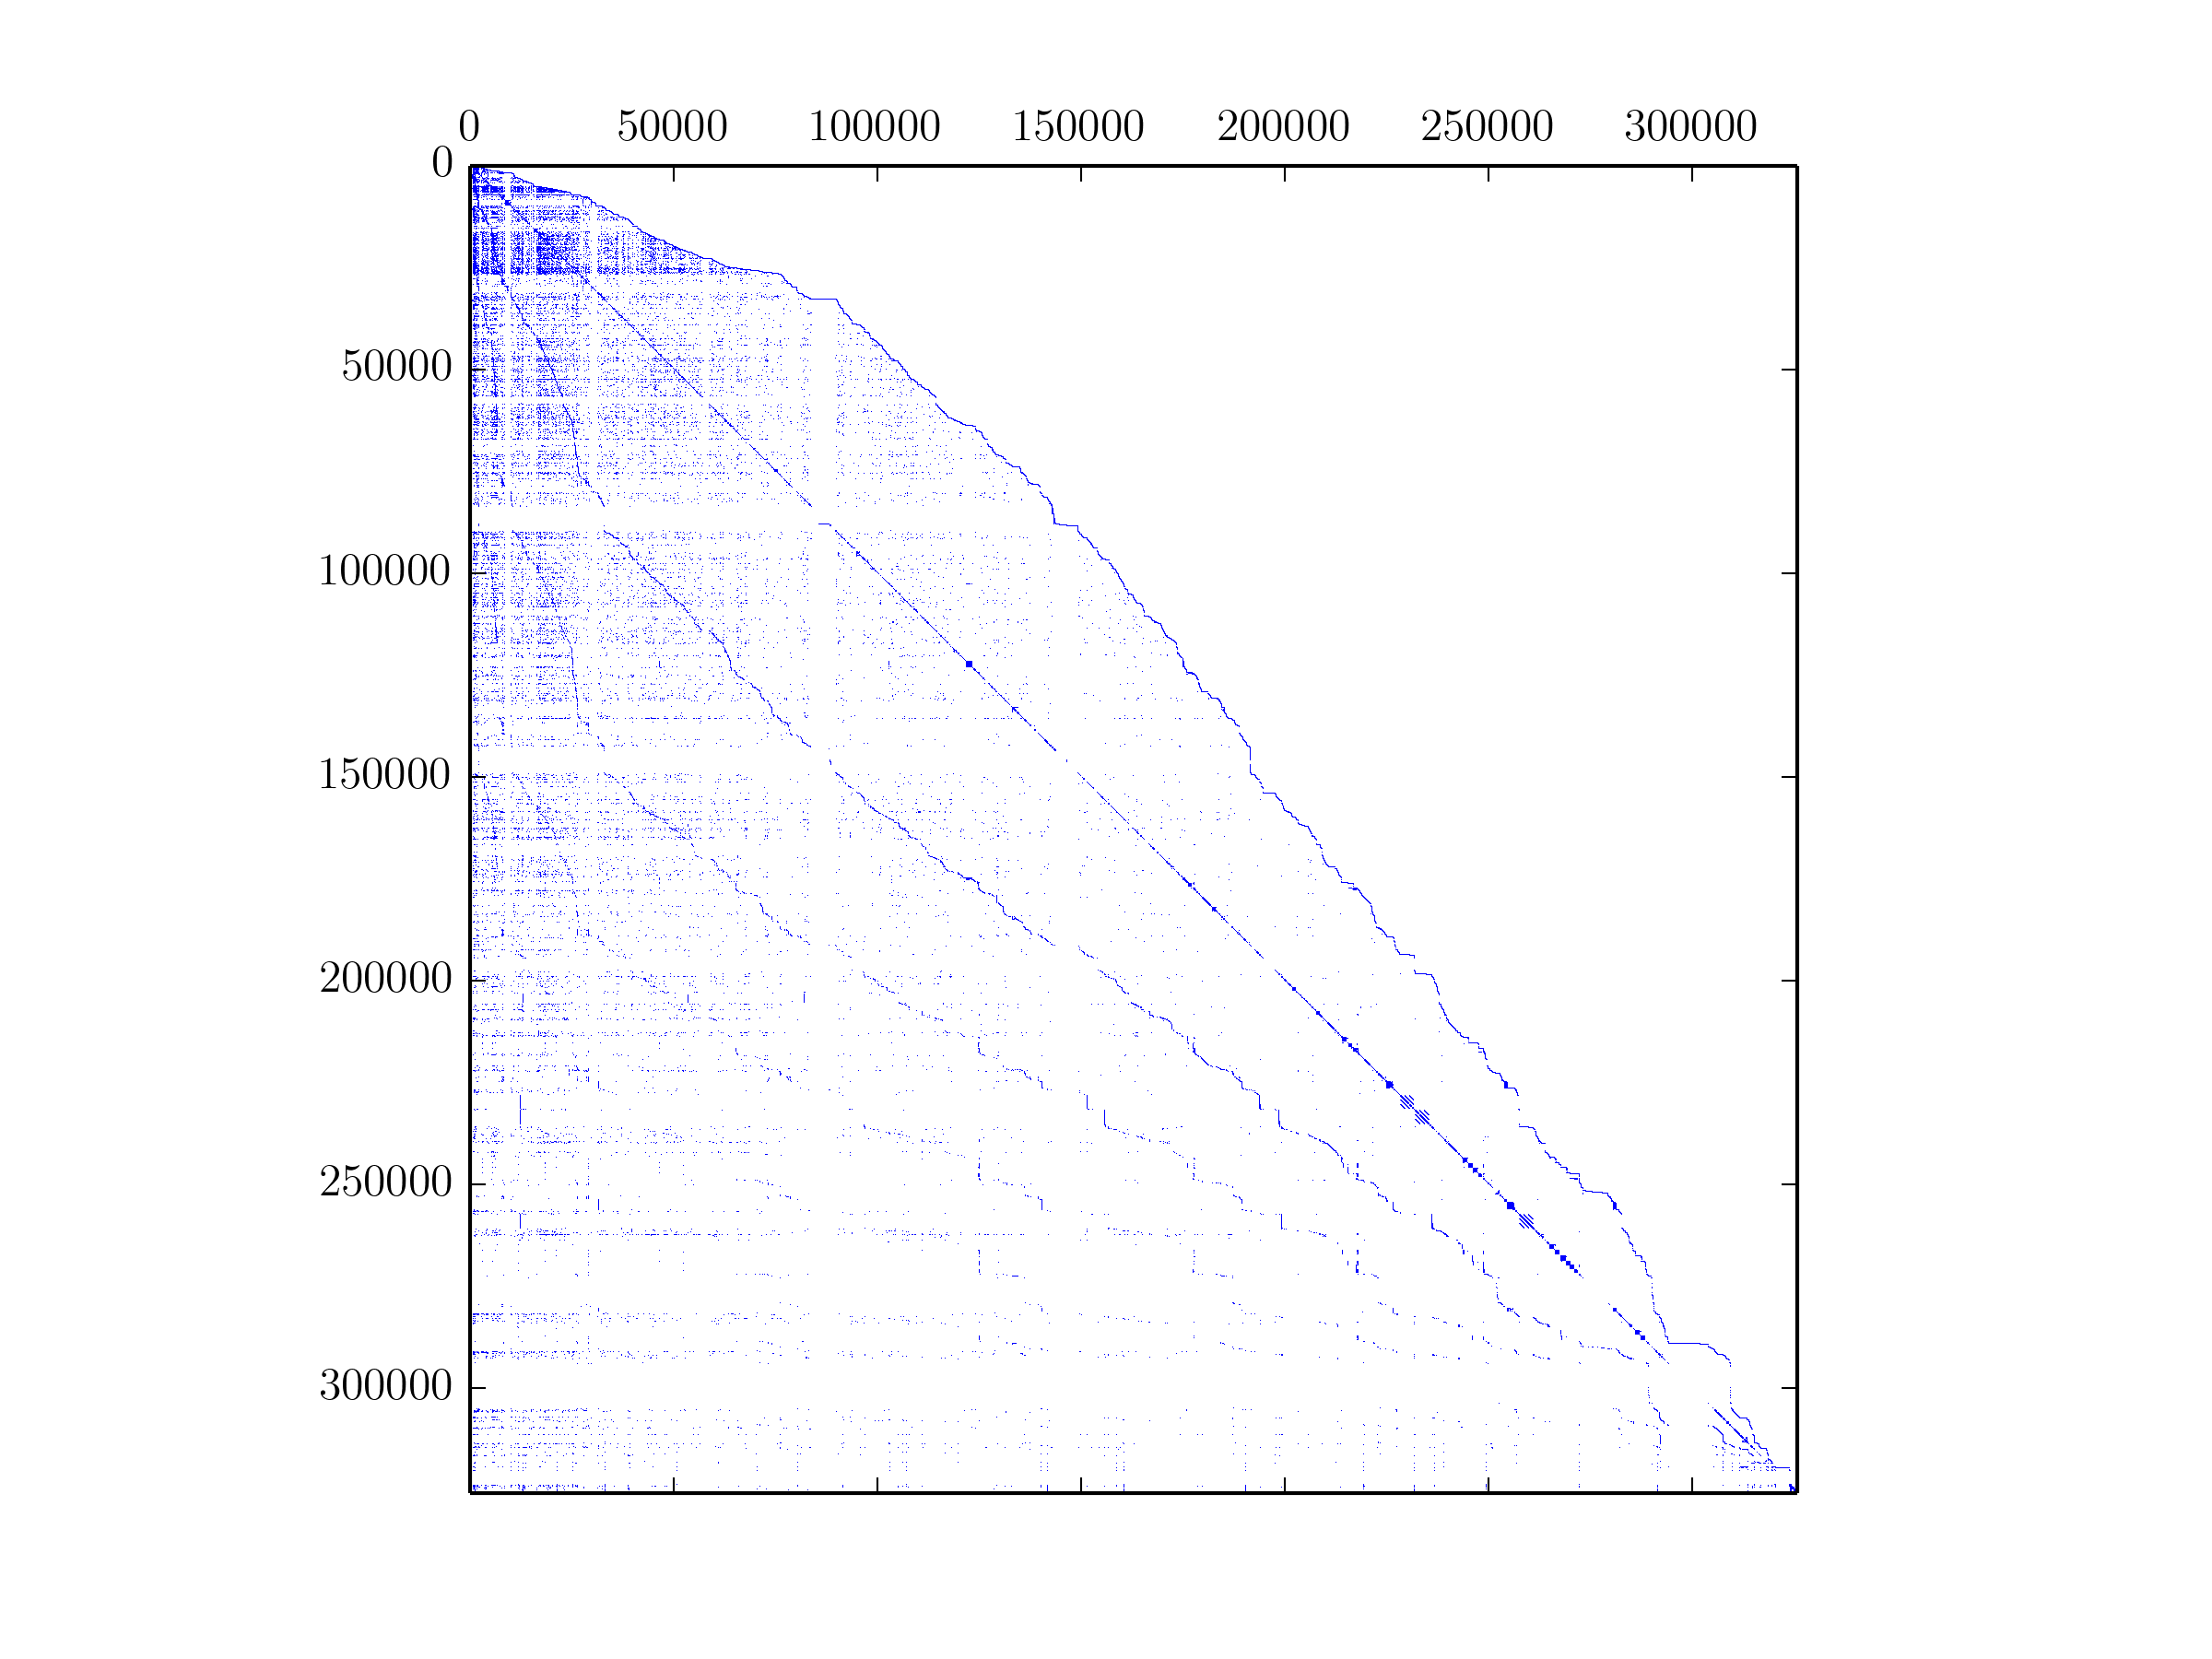
\includegraphics[width=\textwidth]{sparse_web.png}
\caption{Output of the \li{spy} command on the adjacency matrix corresponding to the websites supported by Notre Dame University in 1999.
Data was taken from the SNAP datasets.}
\label{fig:WebSparse}
\end{figure}
\end{comment}

\begin{problem}
(Optional) Try running the functions you wrote in this lab on a data set downloaded from SNAP.
\begin{enumerate}
\item Begin by running your methods on the first 100 nodes of the data set.
\item Modify your solution to Problem \ref{prob:pagerank_dense_iter} so that it uses only sparse matrices. 
With this modification, you should be able to run the function on more nodes.
Hint: Convert the adjacency matrix to a \li{csc_matrix} or a \li{csr_matrix} to perform the computations.
\end{enumerate}
\end{problem}
